\documentclass[12pt]{beamer}
\usepackage{pgf}
\usepackage[danish]{babel}
\usepackage[utf8]{inputenc}
\usepackage{beamerthemesplit}
\usepackage{graphics,epsfig, subfigure}
\usepackage{url}
\usepackage{srcltx}
\usepackage{hyperref}
\usepackage{fancybox}
\usepackage{listings}
\lstset{
  language=C,                % choose the language of the code
   basicstyle=\footnotesize,        % the size of the fonts that are used for the code
    keywordstyle=\color{blue},       % keyword style
     commentstyle=\color[rgb]{0.13,0.54,0.13},
  numbers=left,                   % where to put the line-numbers
  stepnumber= 0.3,                   % the step between two line-numbers.        
  numbersep=1pt,                  % how far the line-numbers are from the code
  backgroundcolor=\color{white},  % choose the background color. You must add \usepackage{color}
  showspaces=false,               % show spaces adding particular underscores
  showstringspaces=false,         % underline spaces within strings
  showtabs=false,                 % show tabs within strings adding particular underscores
  tabsize=2,                      % sets default tabsize to 2 spaces
  captionpos=b,                   % sets the caption-position to bottom
  breaklines=true,                % sets automatic line breaking
  breakatwhitespace=true,         % sets if automatic breaks should only happen at whitespace
 % title=\lstname,                 % show the filename of files included with \lstinputlisting;
}
\definecolor{kugreen}{RGB}{50,93,61}
\definecolor{kugreenlys}{RGB}{132,158,139}
\definecolor{kugreenlyslys}{RGB}{173,190,177}
\definecolor{kugreenlyslyslys}{RGB}{214,223,216}
\setbeamercovered{transparent}
\mode<presentation>
\usetheme[numbers,totalnumber,compress,sidebarshades]{PaloAlto}
\setbeamertemplate{section in toc}[sections numbered]

\setbeamertemplate{footline}[frame number]

  \usecolortheme[named=kugreen]{structure}
  \useinnertheme{circles}
  \usefonttheme[onlymath]{serif}
  \setbeamercovered{transparent}
  \setbeamertemplate{blocks}[rounded][shadow=true]

\logo{
\includegraphics[width=0.8cm]{fga_logo.png}}
%\useoutertheme{infolines} 
\title{GPP-MDS}
\subtitle{Projeto guiado por comportamento e Histórias de usuário}
\author{Carla Rocha, Hilmer R. Neri}


\institute{Engenharia de Software \\ Universidade de Brasília}
\date{}


\begin{document}
\frame{\titlepage \vspace{-0.5cm}	
}
\frame
{
\frametitle{Scrum}
\tableofcontents%[pausesection]
}
\begin{frame}
\frametitle{Filosofia R2}
 \begin{block}{}
  "Use a estatística/indicadores/métricas como o bêbado usa o poste:
  mais pelo apoio que pela iluminação" (Adaptação Andrew Lang)
 \end{block}
\end{frame}

\begin{frame}
 \begin{block}{Bom desenvolvedor}
  Ser um bom desenvolvedor vai muito além de conhecer muitas linguagens de programação ou conhecer em detalhe o funcionamento de uma delas.
  Ser um bom desenvolvedor é mais do que dominar um assunto e virar uma referência nele. É mais do que saber escrever de cabeça a melhor
  regex para reconhecer um endereço de email. Ser um bom desenvolvedor, para mim, é se importar genuinamente com a qualidade de tudo
  que se está desenvolvendo e entregando, em todas as fases. Nessa visão o trabalho não está concluído quando o código foi pro ar, ele 
  apenas entra em uma nova fase onde devemos mais uma vez conseguir entender que o que estamos entregando faz sentido e tem qualidade.
 \end{block}
\footnote{Fonte:http://shipit.resultadosdigitais.com.br/blog/tdd-testes-depois-do-deploy/}
\end{frame}

\begin{frame}
 \begin{block}{Bom desenvolvedor se preocupa com a qualidade}
 \begin{itemize}
  \item Aspectos funcionais
  \item Aspectos técnicos: Sistemas de apoio
  \item Aspectos tecnicos: Performance
  \item Aspectos de uso
 \end{itemize}

 \end{block}
\footnote{Fonte:http://shipit.resultadosdigitais.com.br/blog/tdd-testes-depois-do-deploy/}
\end{frame}

\begin{frame}
 \frametitle{Manifesto Agil}
  \begin{figure}
   \centering
   
\includegraphics[width = \textwidth]{figs/manifesto.jpg}
  \end{figure}
\end{frame}


\begin{frame}
 \frametitle{Juramento do Programador}
  \begin{figure}
   \centering
   
\includegraphics[height = \textheight]{figs/theprogrammersoath.png}
  \end{figure}
\end{frame}

\begin{frame}
 \frametitle{Manifesto Software Artesanal}
  \begin{figure}
   \centering
   
\includegraphics[height = \textheight]{figs/SCManifesto.jpg}
  \end{figure}
\end{frame}

\section{Scrum - Empirismo}
\begin{frame}
 \frametitle{Scrum}
 \begin{block}{Definição}
  Scrum é um \textit{framework} estrutural que está sendo usado para gerenciar o desenvolvimento de
produtos complexos desde o início de 1990
 \end{block}
\end{frame}

 \begin{frame}
 \frametitle{Scrum}
  \begin{itemize}
   \item O framework Scrum consiste nos times do Scrum associadas a papéis, eventos, artefatos e
regras 
\item Cada componente dentro do framework serve a um propósito específico e é essencial
para o uso e sucesso do Scrum
\item As regras do Scrum integram os eventos, papéis e artefatos, administrando as relações e
interações entre eles.
  \end{itemize}
 \end{frame}
 


\begin{frame}
 \frametitle{Scrum - Teoria do Scrum}
 \begin{itemize}
  \item É fundamentado nas teorias empíricas de controle de processo, ou empirismo
  \item O empirismo afirma que o conhecimento vem da experiência e de tomada de
decisões baseadas no que é conhecido
\item O Scrum emprega uma abordagem iterativa e
incremental para aperfeiçoar a previsibilidade e o controle de riscos
 \end{itemize}
\end{frame} 


\begin{frame}
 \frametitle{Scrum - Processo empírico}
 \begin{itemize}
  \item Três pilares apoiam a implementação de controle de processo empírico:
  \begin{enumerate}
   \item \textbf{Transparência} - linguagem compartilhada, definição de "Pronto"
   \item \textbf{Inspeção} - detecção de variações dos artefatos Scrum
   \item \textbf{Adaptação} - mais breve possível para minimizar desvios
  \end{enumerate}
 \end{itemize}
\end{frame} 


\section{Scrum - Framework}
\begin{frame}
 \frametitle{Scrum framework}
  \begin{figure}
   \centering
   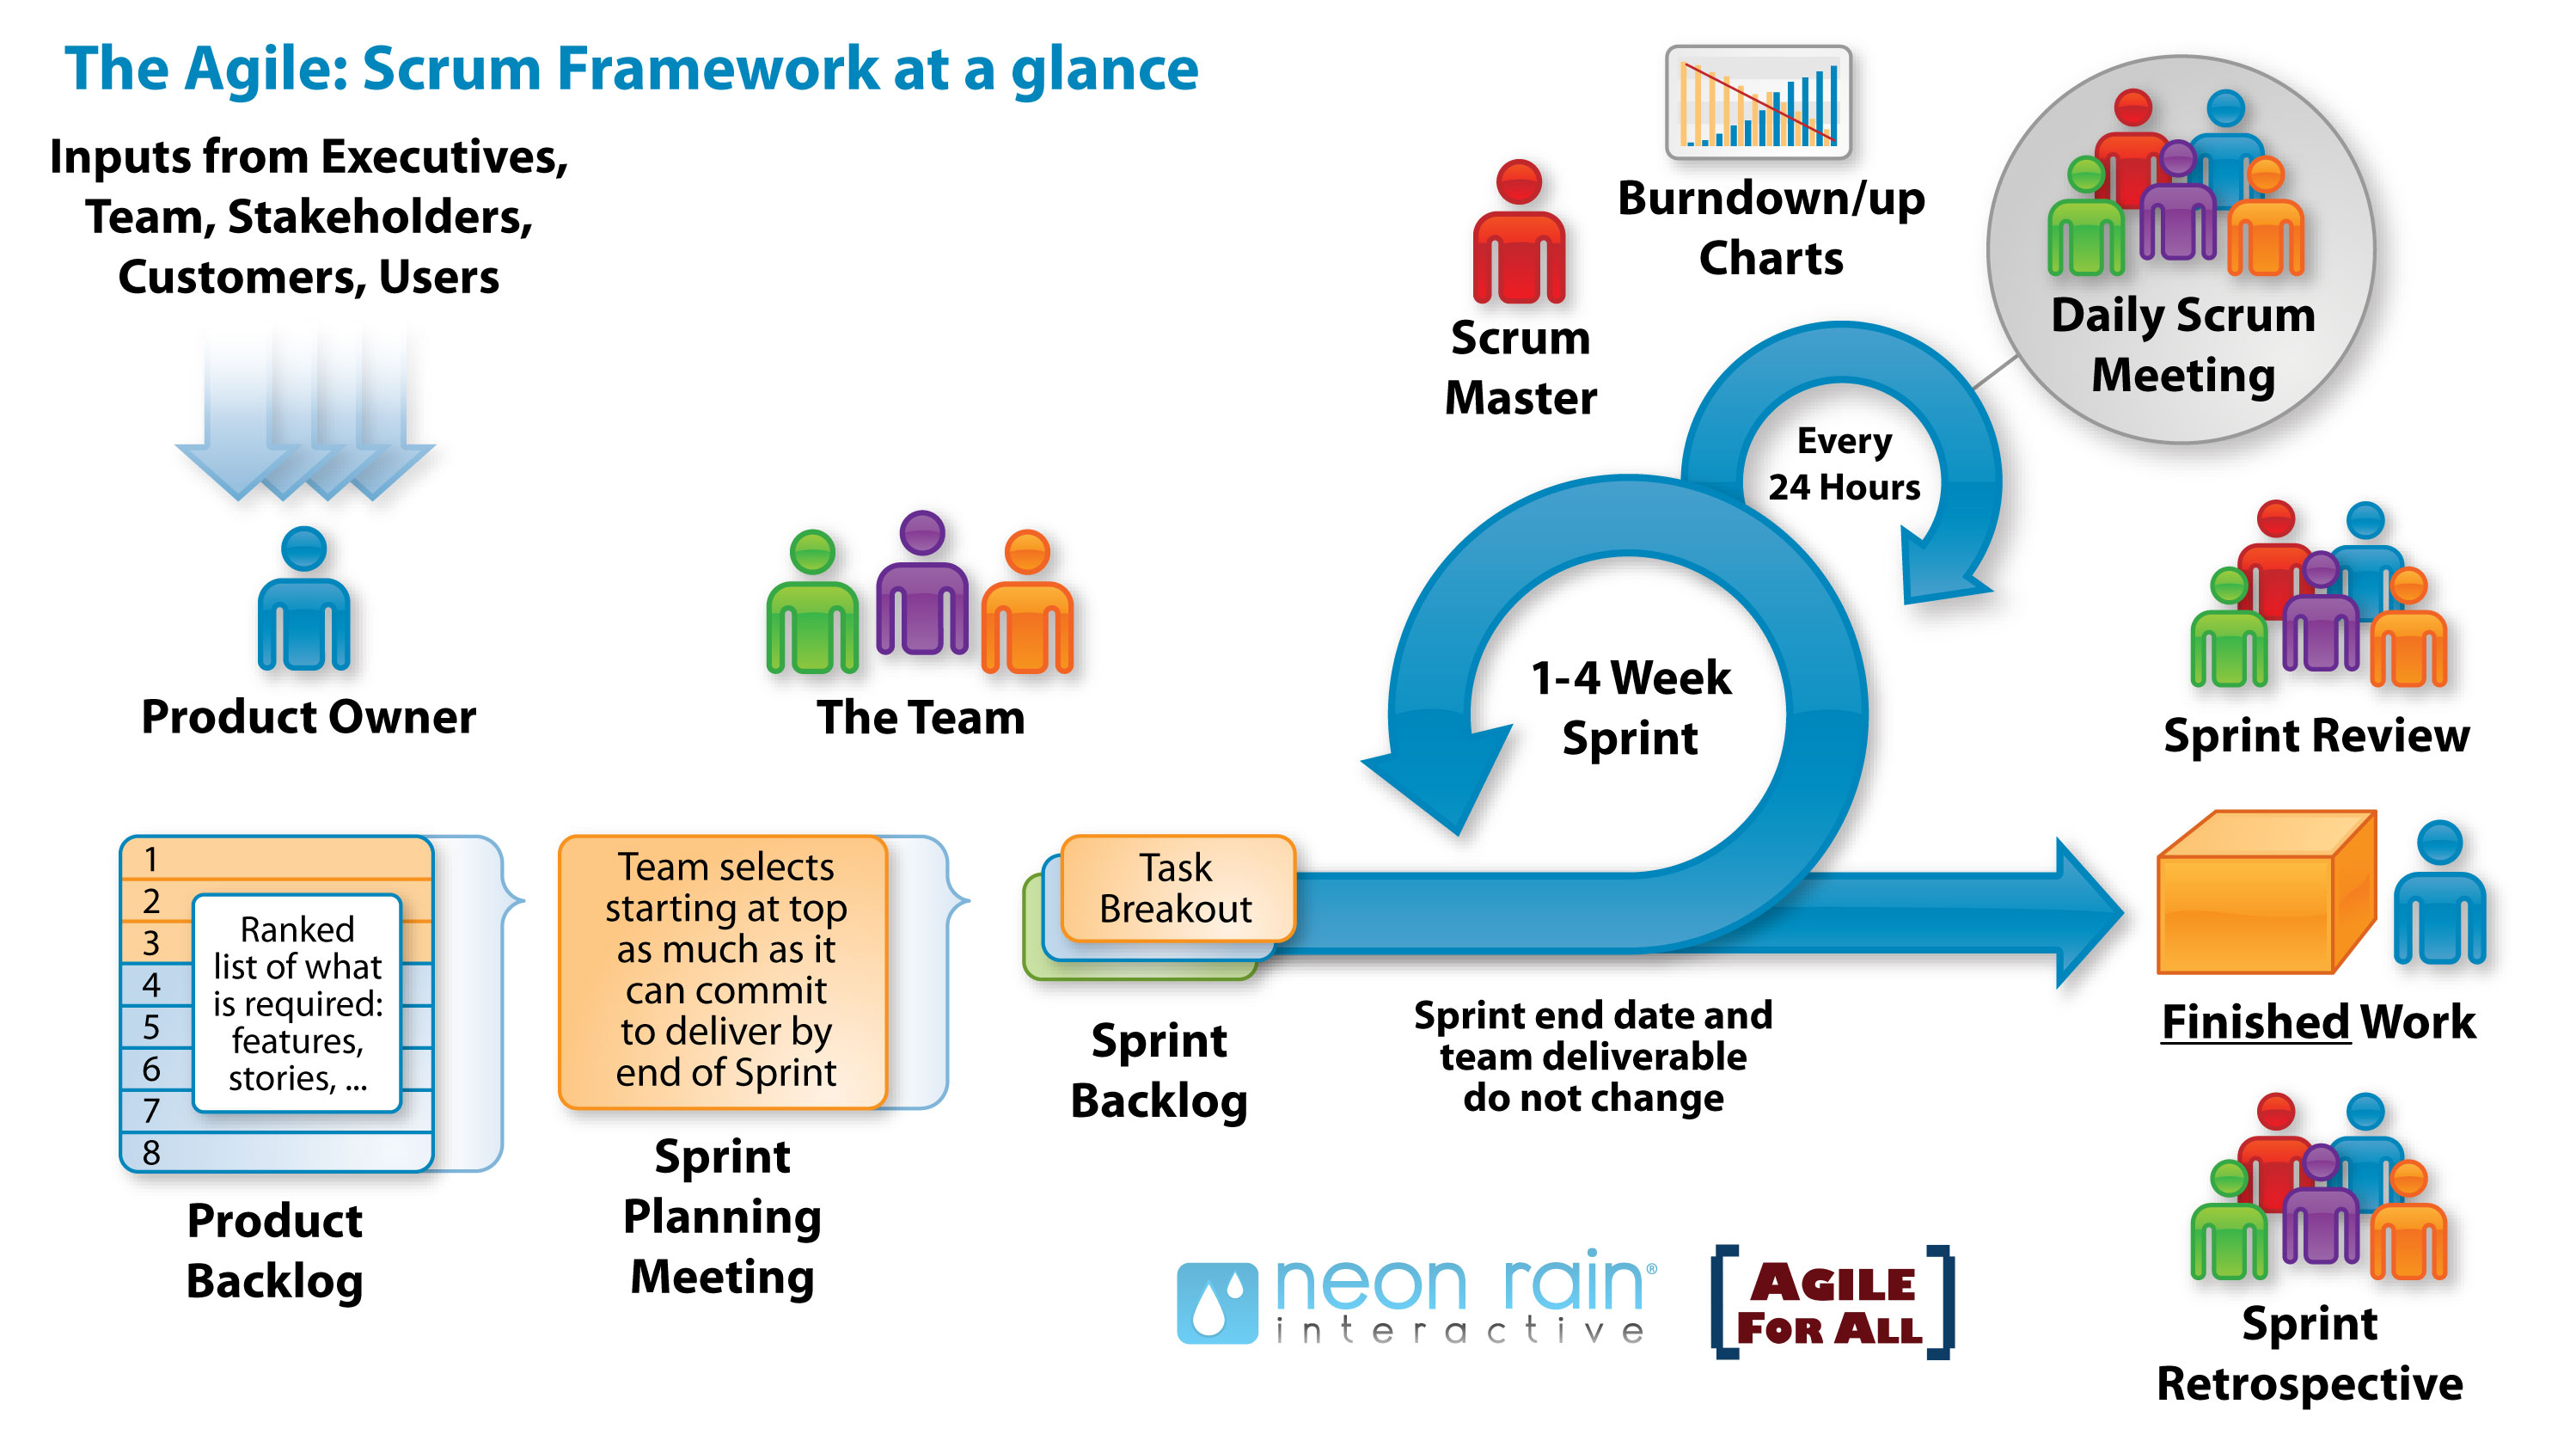
\includegraphics[width = 0.9\textwidth]{figs/Scrum.jpg}
  \end{figure}
\end{frame}

\begin{frame}
 \frametitle{Scrum framework -  Planejamento}
  \begin{figure}
   \centering
   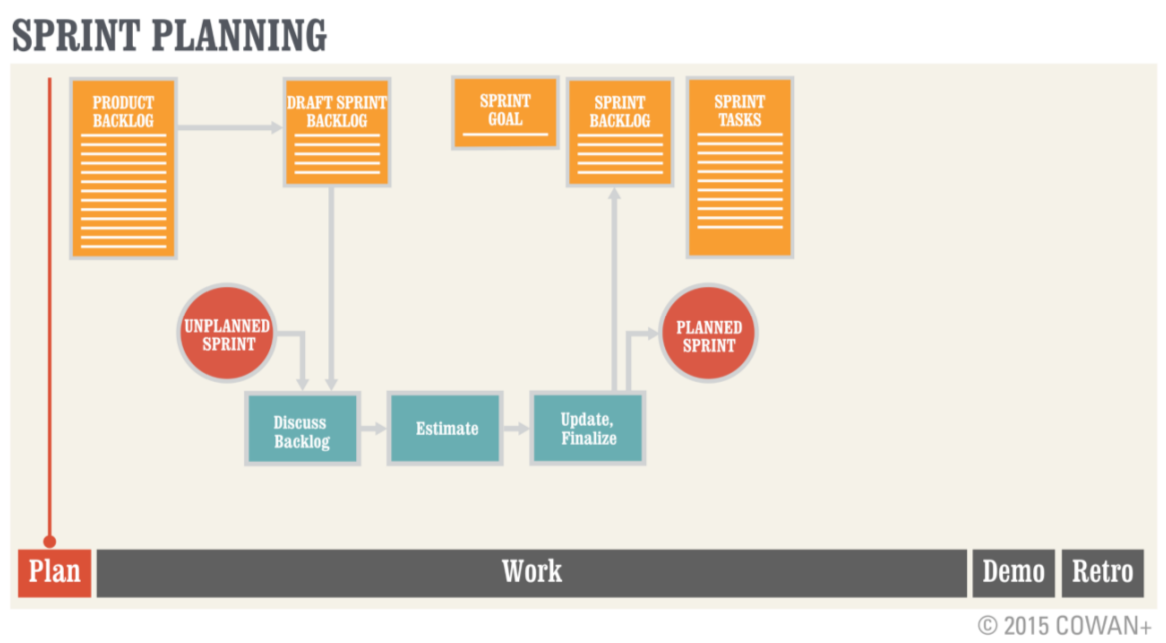
\includegraphics[width =\textwidth]{figs/fases_sprint_planning.png}
  \end{figure}
\end{frame}

\begin{frame}
 \frametitle{Scrum framework -  Execuçao}
  \begin{figure}
   \centering
   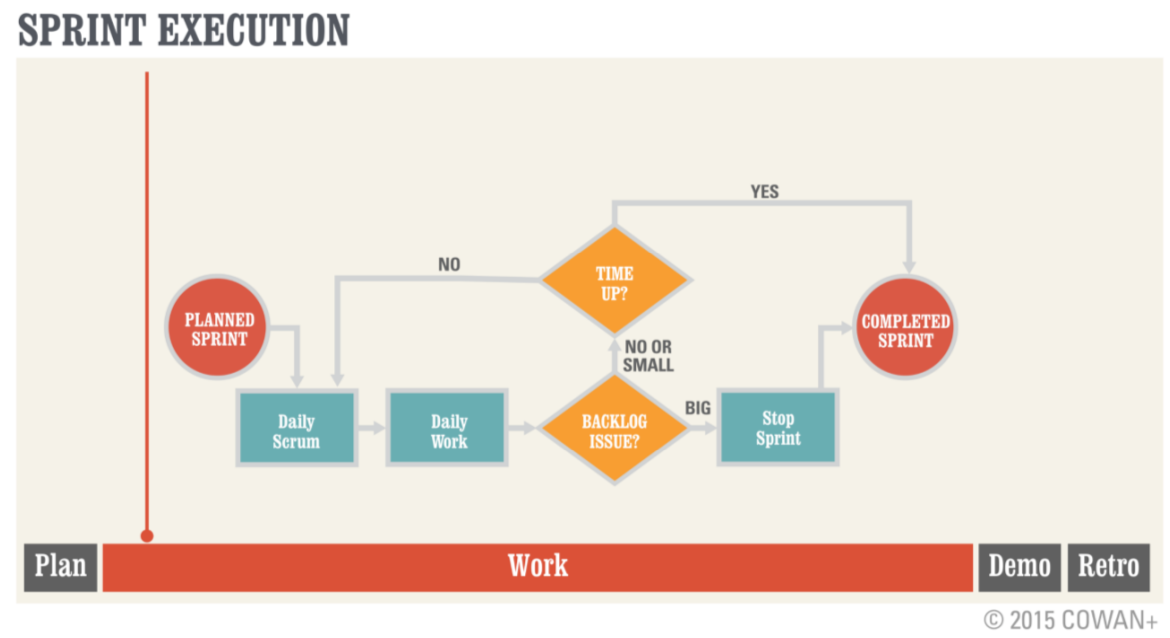
\includegraphics[width = \textwidth]{figs/fases_sprint_execution.png}
  \end{figure}
\end{frame}

\begin{frame}
 \frametitle{Scrum framework -  Demo}
  \begin{figure}
   \centering
   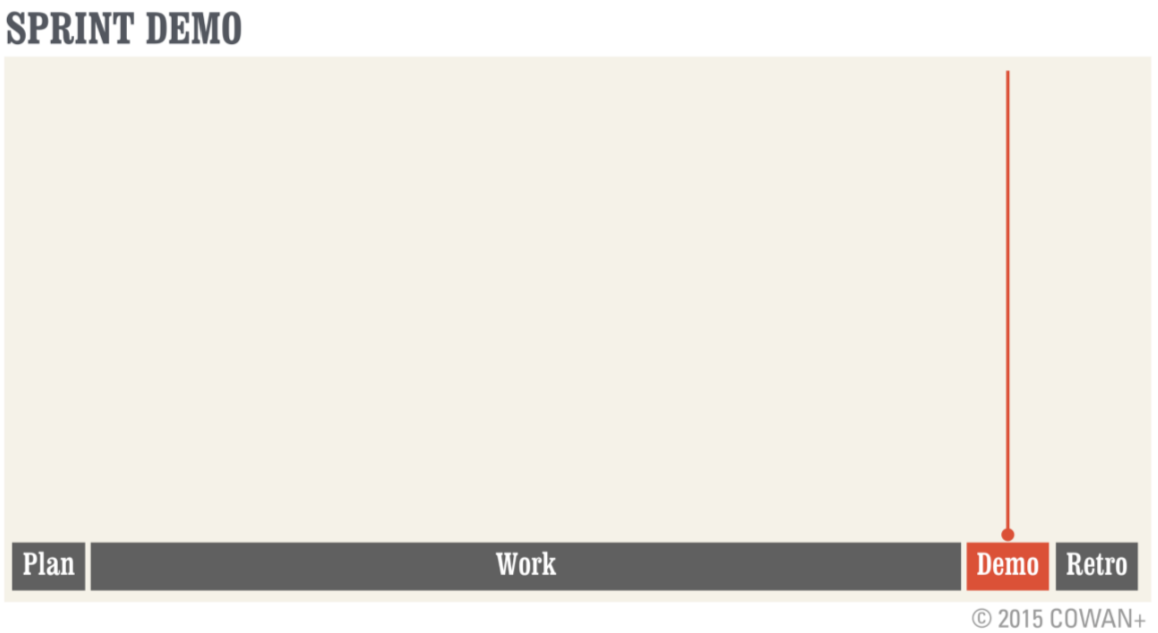
\includegraphics[width = \textwidth]{figs/fases_sprint_demo.png}
  \end{figure}
\end{frame}

\begin{frame}
 \frametitle{Scrum framework -  Retrospectiva}
  \begin{figure}
   \centering
   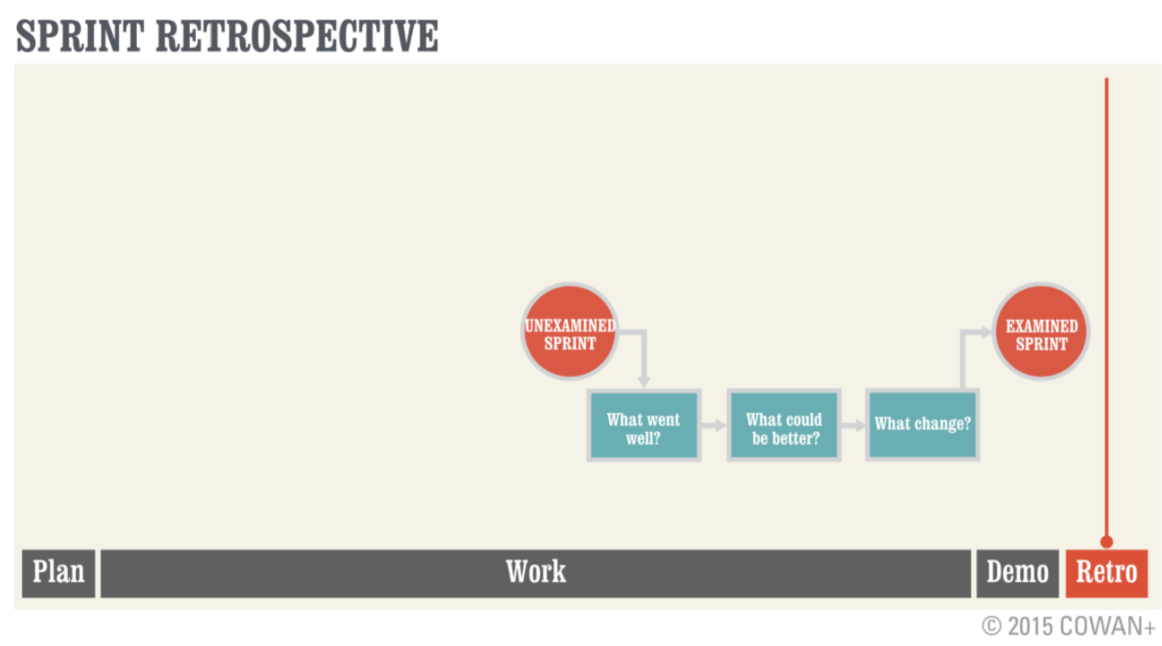
\includegraphics[width = \textwidth]{figs/fases_sprint_retrospective.png}
  \end{figure}
\end{frame}

\begin{frame}
 \frametitle{Scrum framework -  BurnDown}
  \begin{figure}
   \centering
   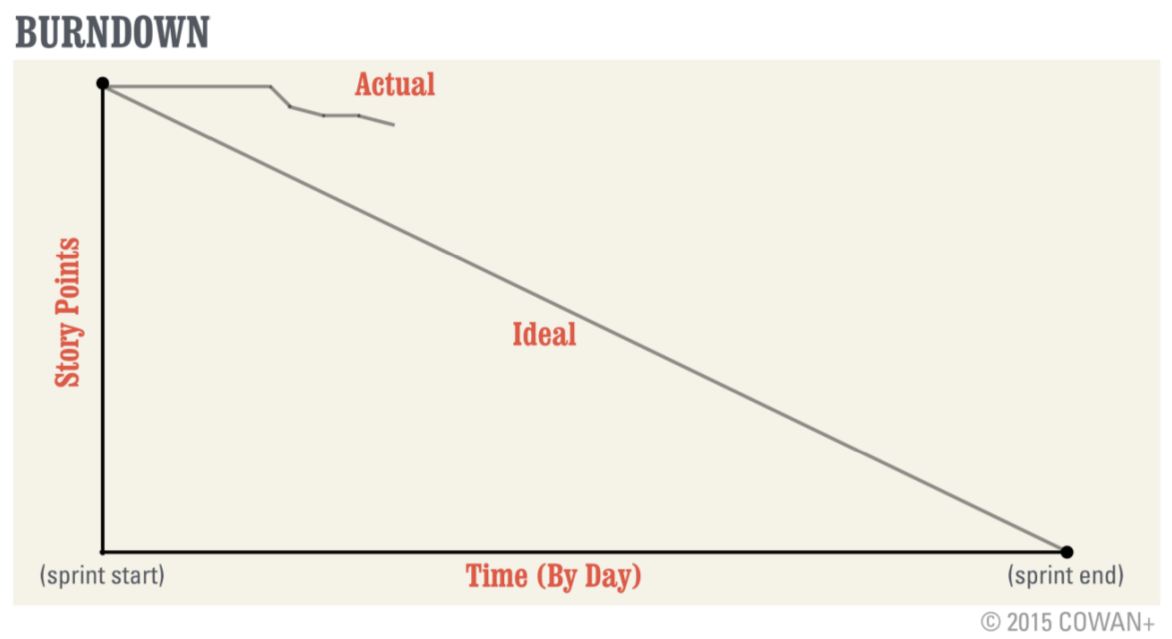
\includegraphics[width = \textwidth]{figs/fases_burndown.png}
  \end{figure}
\end{frame}

\begin{frame}
 \frametitle{Scrum framework -  BurnDown}
  \begin{figure}
   \centering
   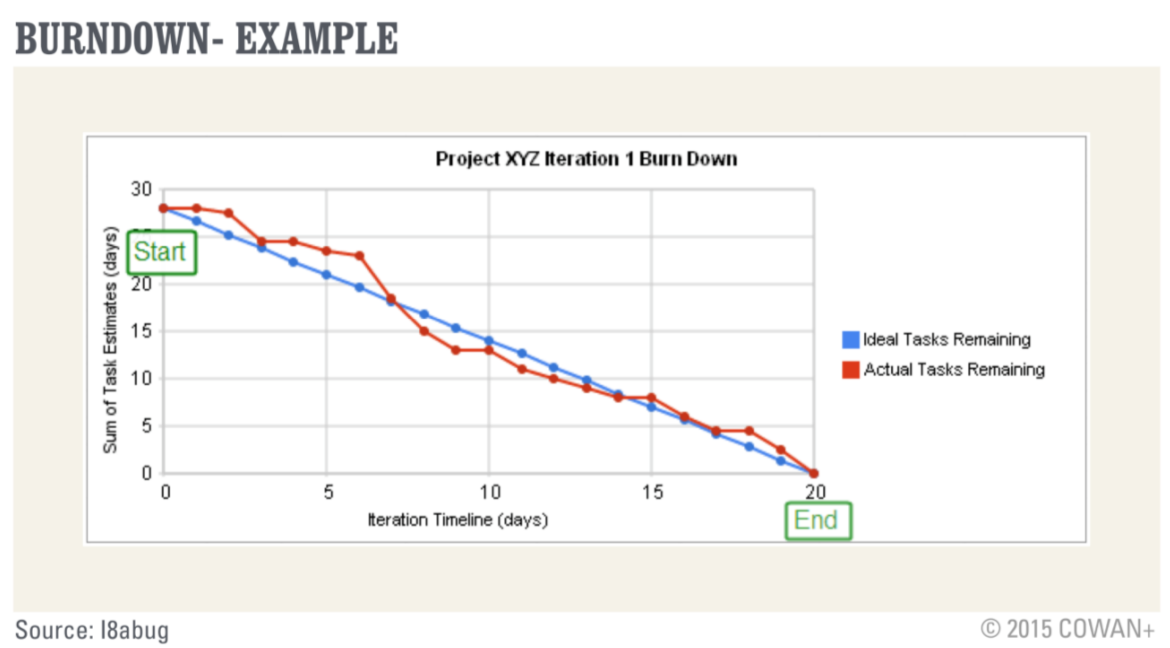
\includegraphics[width = \textwidth]{figs/fases_burndown_exemplo.png}
  \end{figure}
\end{frame}

\section{Scrum - Papéis}
\begin{frame}
 \frametitle{Primeiro Passo: formar e organizar equipe}
 \begin{itemize}
  \item Tamanho ideal da equipe: \textbf{equipe de duas pizzas}:
  \begin{itemize}
   \item Grupo que pode ser alimentado por duas pizzas em um encontro
  \end{itemize}
 \end{itemize}
\end{frame}

\begin{frame}
 \frametitle{Scrum - Papéis}
  \begin{figure}
   \centering
   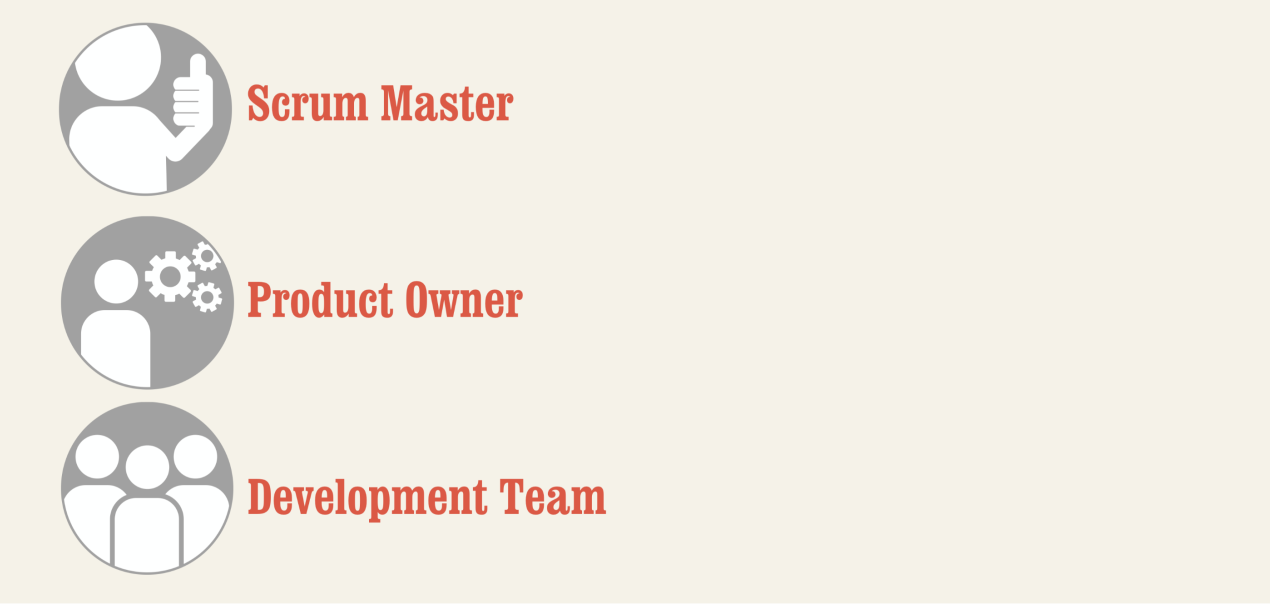
\includegraphics[width = 0.9\textwidth]{figs/scrum_papeis.png}
  \end{figure}
\end{frame}

\begin{frame}
 \frametitle{Papeis}
 \begin{itemize}
  \item Há 3 papéis no scrum
  \begin{enumerate}
   \item Product Owner - Única pessoa responsável pelo gerenciamento do Product Backlog e por garantir o valor do trabalho realizado pelo Time
   \item ScrumMaster - Responsável por garantir que o time de scrum esteja aderindo aos valores Scrum, às práticas e as regras
   \item Time - Transformam o Product Backlog em incrementos de funcionalidades potencialmente entregáveis em cada Sprint
  \end{enumerate}
 \end{itemize}
\end{frame}

\begin{frame}
 \frametitle{Papéis - Product Owner}
 \begin{itemize}
  \item Expressar claramente os itens do Backlog do Produto
  \item Ordenar os itens do Backlog do Produto para alcançar melhor as metas e missões
  \item Garantir o valor do trabalho realizado pelo Time de Desenvolvimento
  \item Garantir que o Backlog do Produto seja visível, transparente, claro para todos, e mostrar o
que o Time Scrum vai trabalhar a seguir
\item Garantir que o Time de Desenvolvimento entenda os itens do Backlog do Produto no nível
necessário
 \end{itemize}
\end{frame}

\begin{frame}
 \frametitle{Papéis - Time de Desenvolvimento}
 \begin{itemize}
  \item Eles são auto-organizados
  \item Times de Desenvolvimento são multifuncionais, possuindo todas as habilidades necessárias,
enquanto equipe, para criar o incremento do Produto
\item O Scrum não reconhece títulos para os integrantes do Time de Desenvolvimento que não
seja o Desenvolvedor
\item Times de Desenvolvimento não contém sub-times dedicados a domínios específicos de
conhecimento
 \end{itemize}
\end{frame}

\begin{frame}
 \frametitle{Scrum Master trabalhando para o Product Owner}
 \begin{itemize}
  \item Encontrando técnicas para o gerenciamento efetivo do Backlog do Produto
  \item Claramente comunicar a visão, objetivo e itens do Backlog do Produto
  \item Ensinar a Time Scrum a criar itens de Backlog do Produto de forma clara e concisa
  \item Compreender a longo-prazo o planejamento do Produto no ambiente empírico
  \item Compreender e praticar a agilidade; e
  \item Facilitar os eventos Scrum conforme exigidos ou necessários.
 \end{itemize}
\end{frame}

\begin{frame}
 \frametitle{Scrum Master trabalhando para o Time de Desenvolvimento}
 \begin{itemize}
  \item Treinar o Time de Desenvolvimento em autogerenciamento e interdisciplinaridade
  \item Ensinar e liderar o Time de Desenvolvimento na criação de produtos de alto valor
  \item Remover impedimentos para o progresso do Time de Desenvolvimento
  \item Facilitar os eventos Scrum conforme exigidos ou necessários
  \item Treinar o Time de Desenvolvimento em ambientes organizacionais nos quais o Scrum não é
totalmente adotado e compreendido
 \end{itemize}
\end{frame}

\begin{frame}
 \frametitle{Scrum Master trabalhando para a Organização}
 \begin{itemize}
  \item Liderando e treinando a organização na adoção do Scrum
  \item Planejando implementações Scrum dentro da organização
  \item Ajudando funcionários e partes interessadas a compreender e tornar aplicável o Scrum
  \item Causando mudanças que aumentam a produtividade do Time Scrum
  \item Trabalhando com outros Scrum Masters para aumentar a eficácia da aplicação do Scrum
nas organizações
 \end{itemize}
\end{frame}



\begin{frame}
 \frametitle{Papeis - adequacao do Scrum}
  \begin{figure}
   \centering
   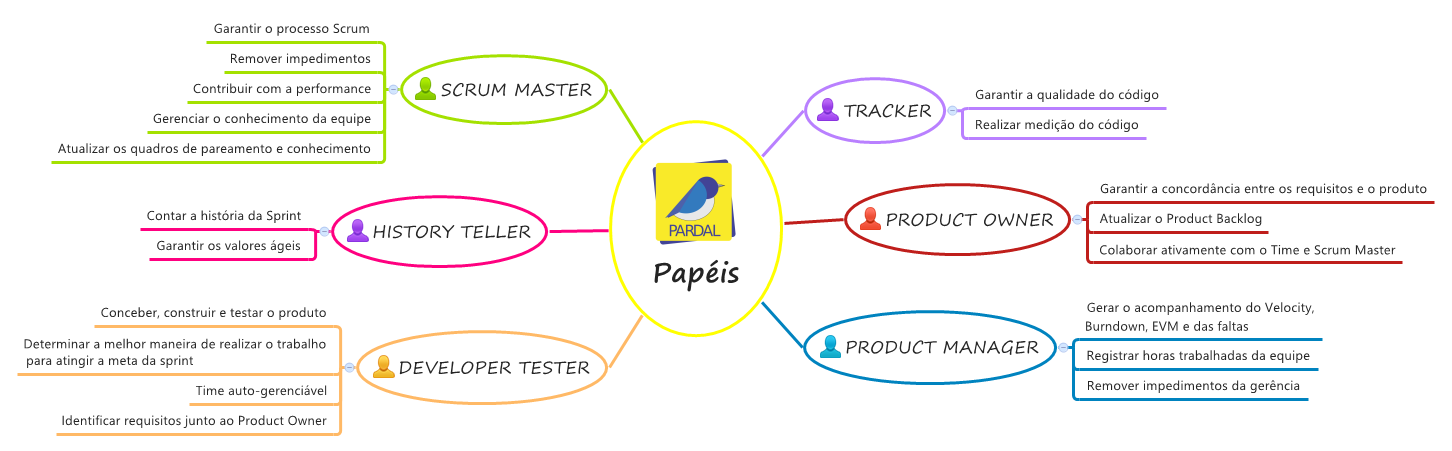
\includegraphics[width = \textwidth]{figs/fig6.png}
  \end{figure}
\end{frame}

\begin{frame}
 \frametitle{Papeis - adequacao do Scrum}
  \begin{figure}
   \centering
   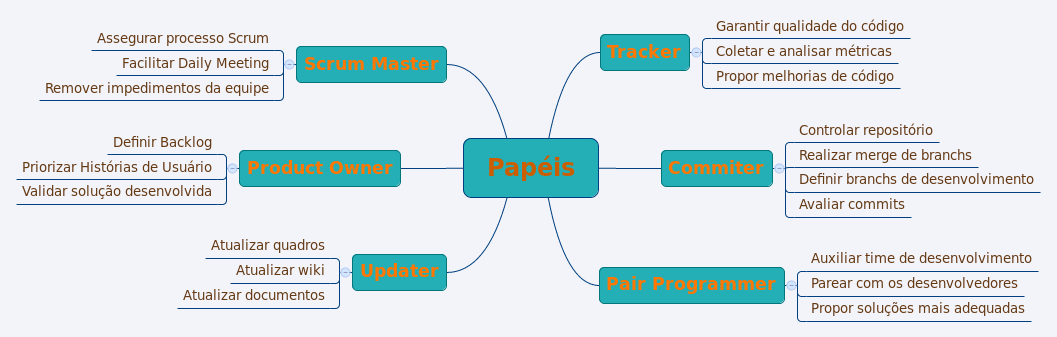
\includegraphics[width = \textwidth]{figs/Papeis2.png}
  \end{figure}
\end{frame}

\begin{frame}
 \frametitle{Papeis - adequacao do Scrum}
  \begin{figure}
   \centering
   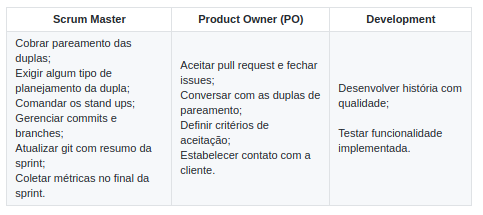
\includegraphics[width = \textwidth]{figs/missaonascente.png}
  \end{figure}
\end{frame}


\section{Scrum - Eventos}

\begin{frame}
 \frametitle{Eventos}
 \begin{block}{Definição}
 Eventos prescritos são usados no Scrum para criar uma rotina e minimizar a necessidade de
reuniões não definidas no Scrum
 \end{block}
  \begin{block}{Característica Principal}
 Todos os eventos são eventos time-boxed, de tal modo que
todo evento tem uma duração máxima
 \end{block}
   \begin{block}{}
Cada evento no Scrum é uma
oportunidade de inspecionar e adaptar alguma coisa
 \end{block}
\end{frame}

\begin{frame}
 \frametitle{Eventos - Sprint}
\begin{block}{Definição}
 A Sprint, um time-boxed de um mês ou menos, durante o qual um
“Pronto”, versão incremental potencialmente utilizável do produto, é criado
 \end{block}
\end{frame}

\begin{frame}
 \frametitle{Eventos - Sprint}
 \begin{itemize}
  \item Cada Sprint pode ser considerada um projeto com horizonte não maior que um mês
  \item Cada Sprint tem a definição do que é para
ser construído, um plano projetado e flexível que irá guiar a construção, o trabalho e o
resultado do produto
\item Sprints também limitam o risco ao custo de um
mês corrido.
 \end{itemize}
\end{frame}

\begin{frame}
 \frametitle{Eventos - Sprint}
 Durante a Sprint
 \begin{itemize}
  \item Não são feitas mudanças que possam por em perigo o objetivo da Sprint;
  \item As metas de qualidade não diminuem; e,
  \item O escopo pode ser clarificado e renegociado entre o Product Owner e o Time de
Desenvolvimento quanto mais for aprendido.
 \end{itemize}
\end{frame}

\begin{frame}
 \frametitle{Eventos - Sprint}
Cancelamento da Sprint
 \begin{itemize}
  \item Somente o Product Owner tem a autoridade para cancelar a Sprint
  \item A Sprint poderá ser cancelada se o objetivo da Sprint se tornar obsoleto
  \item A Sprint deve ser cancelada se ela não faz mais sentido às dadas circunstâncias
  \item Cancelamentos de Sprints são
frequentemente traumáticos para o Time Scrum, e são muito incomuns.
 \end{itemize}
\end{frame}

\begin{frame}
 \frametitle{Eventos - Reunião de Planejamento da Sprint}

 \begin{itemize}
  \item Duração: 2 vezes a quantidade de semanas da sprint (máx. 8 horas)
  \item Deve-se responder as seguintes perguntas:
  \begin{enumerate}
   \item Qual é o objetivo da Sprint?
  \item O que pode ser entregue como resultado do incremento da próxima Sprint?
    \item Como o trabalho necessário para entregar o incremento será realizado?
  \end{enumerate}
 \end{itemize}
\end{frame}

\begin{frame}
 \frametitle{Eventos - Reunião de Planejamento da Sprint}
 Entrada da reunião de planejamento da Sprint
 \begin{itemize}
  \item Backlog do Produto
  \item O mais recente incremento do produto
  \item A capacidade projetada do Time de Desenvolvimento
  \item O desempenho passado do Time de Desenvolvimento
 \end{itemize}
\end{frame}

\begin{frame}
 \frametitle{Eventos - Reunião de Planejamento da Sprint}
Regras
 \begin{itemize}
  \item O número de itens selecionados do Backlog do Produto para a Sprint é o único trabalho do Time de Desenvolvimento
  \item Somente o Time de Desenvolvimento pode avaliar o que pode ser completado ao longo da próxima Sprint
  \item O Time Scrum determina a meta da Sprint
 \end{itemize}
\end{frame}


\begin{frame}
 \frametitle{Eventos - Reunião de Planejamento da Sprint}
Como o trabalho escolhido está Pronto
 \begin{itemize}
  \item O trabalho planejado pelo Time de Desenvolvimento para os primeiros dias da Sprint, este é decomposto até o final desta
reunião, frequentemente em unidades de um dia de duração ou menos
\item o Time de Desenvolvimento deve ser capaz de explicar ao Product Owner e ao Scrum Master como pretende trabalhar como equipe auto-organizada
para completar o objetivo da Sprint e criar o incremento previsto
 \end{itemize}
\end{frame}

\begin{frame}
 \frametitle{Eventos - Reunião Diária}
\begin{block}{Definição}
 A Reunião Diária do Scrum é um evento time-boxed de 15 minutos, para que o Time de
Desenvolvimento possa sincronizar as atividades e criar um plano para as próximas 24 horas.
 \end{block}
 \begin{block}{}
  A Reunião Diária é mantida no mesmo horário e local todo dia para reduzir a complexidade
 \end{block}
\end{frame}

\begin{frame}
 \frametitle{Eventos - Reunião Diária}
\begin{block}{Benefício}
Reuniões Diárias melhoram as comunicações, eliminam outras reuniões, identificam e
removem impedimentos para o desenvolvimento, destacam e promovem rápidas tomadas de
decisão, e melhoram o nível de conhecimento do Time de Desenvolvimento. Esta é uma
reunião chave para inspeção e adaptação.
 \end{block}

\end{frame}


\begin{frame}
 \frametitle{Eventos - Reunião Diária}
Durante a reunião os membros do Time de Desenvolvimento esclarecem
 \begin{itemize}
  \item O que eu fiz ontem que ajudou o Time de Desenvolvimento a atender a meta da Sprint?
  \item O que eu farei hoje para ajudar o Time de Desenvolvimento atender a meta da Sprint?
  \item  Eu vejo algum obstáculo que impeça a mim ou o Time de Desenvolvimento no atendimento
da meta da Sprint?
 \end{itemize}
\end{frame}


\begin{frame}
 \frametitle{Eventos - Reunião Diária}
 \begin{itemize}
  \item O Scrum Master assegura que o Time de Desenvolvimento tenha a reunião, mas
  \item o Time de Desenvolvimento é responsável por conduzir a Reunião Diária
  \item O Scrum Master ensina o Time de Desenvolvimento a manter a Reunião Diária dentro do time-box de 15 minutos
  \item O Scrum Master reforça a regra de que somente os integrantes do Time de Desenvolvimento
participem da Reunião Diária
 \end{itemize}
\end{frame}

\begin{frame}
 \frametitle{Eventos - Revisão da Sprint}
\begin{block}{Definição}
 A reunião de Revisão da Sprint é executada no final da Sprint para inspecionar o incremento e adaptar o
Backlog do Produto se necessário
 \end{block}
 \begin{block}{}
Esta é uma reunião informal, não uma reunião de status
 \end{block}
\end{frame}

\begin{frame}
 \frametitle{Eventos - Revisão da Sprint}
 \begin{itemize}
  \item Os participantes incluem o Time Scrum e os Stakeholders chaves convidados pelo Product
Owner
  \item O Product Owner esclarece quais itens do Backlog do Produto foram “Prontos” e quais não
foram “Prontos”
  \item O Time de Desenvolvimento discute o que foi bem durante a Sprint, quais problemas
ocorreram dentro da Sprint, e como estes problemas foram resolvidos
  \item O Time de Desenvolvimento demonstra o trabalho que está “Pronto” e responde as
questões sobre o incremento
 \end{itemize}
\end{frame}

\begin{frame}
 \frametitle{Eventos - Revisão da Sprint}
 \begin{itemize}
\item O Product Owner discute o Backlog do Produto tal como está. Ele (ou ela) projeta as
prováveis datas de conclusão baseado no progresso até a data (se necessário)
\item O grupo todo colabora sobre o que fazer a seguir, e é assim que a Reunião de Revisão da
Sprint fornece valiosas entradas para a Reunião de Planejamento da próxima Sprint
\item Análise de como o mercado ou o uso potencial do produto pode ter mudado e o que é a
coisa mais importante a se fazer a seguir; e
\item Análise da linha do tempo, orçamento, potenciais capacidades, e mercado para a próxima
versão esperada do produto
 \end{itemize}
\end{frame}

\begin{frame}
 \frametitle{Eventos - Retrospectiva da Sprint}
\begin{block}{Definição}
A Retrospectiva da Sprint é uma oportunidade para o Time Scrum inspecionar a si próprio e
criar um plano para melhorias a serem aplicadas na próxima Sprint
 \end{block}
 \begin{block}{}
Time-boxed de três horas para sprint de um mês
 \end{block}
\end{frame}

\begin{frame}
 \frametitle{Eventos - Retrospectiva da Sprint}
 Objetivos
 \begin{itemize}
  \item Inspecionar como a última Sprint foi em relação às pessoas, aos relacionamentos, aos
processos e às ferramentas
  \item Identificar e ordenar os principais itens que foram bem e as potenciais melhorias; e,
  \item Criar um plano para implementar melhorias no modo que o Time Scrum faz seu trabalho;
 \end{itemize}
\end{frame}

\begin{frame}
 \frametitle{Eventos - Retrospectiva da Sprint}
 \begin{itemize}
  \item O Scrum Master encoraja o Time Scrum a melhorar, dentro do processo do framework do
Scrum, o processo de desenvolvimento e as práticas para fazê-lo mais efetivo e agradável
  \item o Time Scrum planeja formas de
aumentar a qualidade do produto, adaptando a definição de “Pronto” quando apropriado
  \item A Retrospectiva da Sprint
fornece um evento dedicado e focado na inspeção e adaptação
 \end{itemize}
\end{frame}

\section{Scrum - Artefatos}

\begin{frame}
 \frametitle{Artefatos do Scrum}
\begin{block}{Definição}
Os artefatos do Scrum representam o trabalho ou o valor para o fornecimento de
transparência e oportunidades para inspeção e adaptação
 \end{block}
 \begin{block}{}
São especificamente projetados para maximizar a transparência das informações chave
 \end{block}
\end{frame}

\begin{frame}
 \frametitle{Scrum - Funcionalidade "Pronta"}
 \begin{itemize}
  \item Uma funcionalidade "Pronta", significa:
  \begin{enumerate}
   \item Claramente codificada
   \item Refatorada
   \item Suite de testes automatizados (unitário, funcional, ...)
   \item Testes de aceitação
  \end{enumerate}
 \end{itemize}
\end{frame} 

\begin{frame}
 \frametitle{Backlog do Produto}
\begin{block}{Definição}
O Backlog do Produto é uma lista ordenada de tudo que deve ser necessário no produto, e é
uma origem única dos requisitos para qualquer mudança a ser feita no produto
 \end{block}
 \begin{block}{}
 O Backlog do Produto lista todas as características, funções, requisitos, melhorias e correções
que formam as mudanças que devem ser feitas no produto nas futuras versões
 \end{block}
\end{frame}

\begin{frame}
 \frametitle{Backlog do Produto}
 \begin{itemize}
 \item O Product Owner é responsável pelo Backlog do Produto, incluindo seu conteúdo, disponibilidade e
ordenação
  \item Um Backlog do Produto nunca está completo. Documento dinâmico
  \item evolui tanto quanto o produto e o ambiente no qual ele será utilizado evoluem
  \item existirá enquanto o produto também existir
 \end{itemize}
\end{frame}

\begin{frame}
 \frametitle{Backlog do Produto}
 \begin{itemize}
 \item Os itens do Backlog do Produto possuem os atributos de descrição, ordem, estimativa e valor
   \item O Time de Desenvolvimento é responsável por todas as estimativas
  \item Os itens do Backlog do Produto de ordem mais alta (topo da lista) devem ser mais claros e
mais detalhados que os itens de ordem mais baixa
  \item Os itens do Backlog do Produto que irão ocupar o desenvolvimento na próxima
Sprint são mais refinados, de modo que todos os itens possam ser “Prontos” dentro do time-
boxed da Sprint
 \end{itemize}
\end{frame}

\begin{frame}
 \frametitle{Backlog da Sprint}
\begin{block}{Definição}
O Backlog da Sprint é um conjunto de itens do Backlog do Produto selecionados para a Sprint
 \end{block}
 \begin{block}{}
O Backlog da Sprint torna visível todo o trabalho que o Time de Desenvolvimento identifica
como necessário para atingir o objetivo da Sprint
 \end{block}
\end{frame}

\begin{frame}
 \frametitle{Bibliografia da aula}
 \begin{itemize}
 \item Agile Team Management (Coursera) - \url{https://www.coursera.org/learn/agile-team-management}
 \item Construindo Software como Serviço (SaaS): Uma Abordagem Ágil Usando Computação em Nuvem  
 \item Guia Scrum - \url{http://www.ailtonsousa.com.br/wp-content/uploads/2014/07/Scrum-Guide-Portuguese-BR.pdf}
 \item Guia Xp - \url{http://www.cin.ufpe.br/~gamr/FAFICA/Desenvolvimento\%20de\%20sistemas/XP.pdf}
 \end{itemize}
\end{frame}

% 
% \section{Scrum - Monitoramento}
% 
% \begin{frame}
%  \frametitle{Monitorando o progresso a caminho do objetivo}
%  \begin{itemize}
%   \item \textbf{Ponto}: classificação de cada história de usuário, de acordo com sua complexidade de implementação
%   \item \textbf{Velocidade}: a média de \textbf{pontos} por iteração que um grupo completa
%   \item \textbf{Backlog}: é o nome da coleção de histórias que ainda não foram completadas nessa iteração
%  \end{itemize}
% \end{frame}
% 
% \begin{frame}
%  \frametitle{Velocidade}
%  \begin{itemize}
%   \item É a taxa de trabalho baseada em autoavaliação realizada pela própria equipe
%   \item O propósito da velocidade é dar a todos \textit{stakeholders} a ideia de quantas iterações serão necessárias para uma
%   equipe adicionar um conjunto de recursos desejados, o que ajuda a definir expectativas mais razoáveis e reduz as chances de 
%   frustração
%  \end{itemize}
% \end{frame}
% 
% \begin{frame}
%  \frametitle{Auto avaliação}
%  \begin{itemize}
%   \item Ao comparar duas equipes, a que tem mais velocidade é mais produtiva
%   \pause
%   \begin{itemize}
%    \item Falso
%   \end{itemize}
%   \item Quando você não sabe como abordar uma história de usuário, basta atribuir a ela 3 pontos
%   \pause
%   \begin{itemize}
%    \item Falso
%   \end{itemize}
%  \end{itemize}
% \end{frame}
% 
% \begin{frame}
%  \frametitle{Histórias de usuário, pontos e velocidade}
%  \begin{itemize}
%   \item Correspondem a sete grandes tarefas das metodologias planeje-e-documente:
%   \begin{enumerate}
%    \item Levantamento de requisitos
%    \item Documentação de Requisitos
%    \item Estimativa de custo
%    \item Planejamento e acompanhamento do progresso
%   \end{enumerate}
%  \end{itemize}
% \end{frame}
% 
% \begin{frame}
%  \frametitle{Histórias de usuário, pontos e velocidade}
%  \begin{itemize}
%   \item Como requisitos mudam com o passar do tempo, outras tarefas são necessárias
%   \begin{enumerate}
%    \item[5] Gestão de mudanças dos requisitos, custos e cronograma
%    \item[6] Garantir que a implementação corresponda às funcionalidades descritas
%    \item[7] Análise de risco e gestão
%   \end{enumerate}
%  \end{itemize}
% \end{frame}
% 
% 
% \begin{frame}
%  \frametitle{Monitorando}
%  \begin{itemize}
%   \item Em qualquer ponto do tempo, o total de trabalho restante para alcançar o objetivo pode ser somado
%   \item \textit{Product Owner} acompanha o total do trabalho restante pelo menos a cada Reunião de Revisão de Sprint
%   \item \textit{Product Owner} compara este valor com o trabalho restante  na reunião de Revisão de Sprint anterior, para avaliar o progresso
%   \item Toda a informação de monitoramento deve ser transparente a toda a equipe
%   
%  \end{itemize}
% 
% \end{frame}
% 
% 
% \begin{frame}
%  \frametitle{Projeto guiado por comportamento - Método Agil}
%  \begin{block}{}
%   Projeto guiado por comportamento é o Desenvolvimento guiado por testes feito corretamente
%  \end{block}
% \end{frame}
% 
% \begin{frame}
%  \begin{block}{Gerenciamento de Projeto: Scrum}
%   Programação pareada e Sistemas de Controle de versão: "Não há vencedores em uma equipe perdedora,
%   nem perdedores em uma equipe vencedora" (Fred Brooks)
%  \end{block}
%  \end{frame}
%  
% \begin{frame}
%  \frametitle{Iteração do ciclo de vida de um programa Agil}
%   \begin{figure}
%    \centering
%    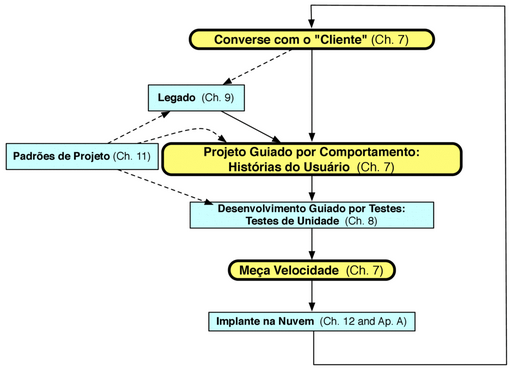
\includegraphics[width = 0.9\textwidth]{figs/fig1.png}
%   \end{figure}
% \end{frame}
% 
% \begin{frame}
%  \frametitle{Ciclo de vida Agil}
%  \begin{itemize}
%   \item Trabalhar de maneira próxima e contínua com os \textit{stakeholders} para desenvolver requisitos e testes
%   \item Manutenção do protótipo funcional enquanto novos produtos são implantados
%   \item O desenvolvimento ágil não troca de fases
%   \item O modo manutenção é presente desde o início da implementação
%  \end{itemize}
% \end{frame}
% 
% \begin{frame}
%  \frametitle{Projeto Guiado por Comportamento (BDD)}
%  \begin{itemize}
%   \item O BDD (\textit{behavior Driven Development}) inicia o ciclo de vida ágil
%   \item O BDD faz questionamento sobre o comportamento  de uma aplicação \textit{antes e durante o desenvolvimento}
%   \item Os requisitos são continuamente aprimorados para assegurar que o software desenvolvido esteja de acordo com a vontade 	dos interessados
%   \item O objetivo dos requisitos do BDD é \textbf{validação} (construir a coisa certa), não apenas \textbf{verificação} (fazer certo a coisa)
%  \end{itemize}
% \end{frame}
% 
% \begin{frame}
%  \frametitle{Projeto Guiado por Comportamento (BDD)}
%  \begin{itemize}
%   \item Em BDD, a versão do conceito de requisitos são histórias de usuários, que descrevem como se espera que a aplicação seja usada
%   \item Histórias de usuário ajudam os \textit{stakeholders} a planejar e priorizar o desenvolvimento
%   \item Ao se concentrar no \textit{comportamento} da aplicação ao invés de se concentrar em sua \textit{implementação},  fica mais fácil reduzir
%   mal-entendidos entre \textit{stakeholders}
%  \end{itemize}
% \end{frame}
% 
% \begin{frame}
%  \frametitle{Histórias de Usuários}
%  \begin{block}{}
%   A vantagens das histórias de usuários e do BDD é criar uma linguagem comum compartilhada entre todos os \textit{stakeholders},
%   especialmente entre os clientes não técnicos
%  \end{block}
% \end{frame}
% 
% \begin{frame}
%  \frametitle{História de usuário}
%  \begin{block}{}
%   História de usuários deve poder ser testadas, ser pequenas o suficiente para que possam ser implementadas em uma iteração e deve possuir valor de negócio
%  \end{block}
% \end{frame}
% 
% \begin{frame}
%  \frametitle{Histórias de usuário - O que faz uma boa história de usuário?}
%  \begin{itemize}
%   \item Acrônimo SMART oferece diretrizes concretas: 
%   \begin{itemize}
%    \item \textit{Specific} - Específico
%    \item \textit{Measurement} - Mensurável
%    \item \textit{Achievable} - Realizável
%    \item \textit{Relevant} - Relevante
%    \item \textit{Timeboxed} - Prazo fixo
%   \end{itemize}
%  \end{itemize}
% \end{frame}
% 
% 


\end{document}
